In this chapter, we discuss the datasets, the baselines, the metrics used, the results and the limitations of ReMLOFT. We used the Debian GNU/Linux Machine, with eight cores and 52GB RAM for the implementation of our approach.

\section{Datasets}
We use the Question Answering over Linked Data (QALD) datasets in our evaluation as QALD\footnote{http://qald.aksw.org/} challenge has established itself as a well-known KGQA competition on DBpedia. For each edition of the challenge, new datasets (benchmarks) for training and testing have been published. QALD includes nine benchmarks from QALD-1 to QALD-9. 

Each question in these datasets is accompanied by a SPARQL query that include the gold standard relations. Due to the evolving nature of knowledge graphs and the fact that they are continuously changing, we filtered the questions in these datasets by running the SPARQL queries against DBpedia to check if they indeed return answers. Questions in the QALD datasets vary in complexity and include simple and complex questions. 

We used the following benchmarks in particular: 

\textbf{QALD-5}  \cite{qald5}: This benchmark consists of over 340 training questions and focuses on multilingual question answering. We restrict our work to questions in English. After filtering, we get 206 questions.

\textbf{QALD-7} \cite{qald7}: The training data consists of 215 questions compiled and curated from previous challenges. The questions vary based on their complexity, including questions with counts (e.g., \textit{How many languages are spoken in Colombia?}), superlatives (e.g., \textit{Which Indian company has the most employees?}), comparatives (e.g., \textit{Give me all books by William Goldman with more than 300 pages.}), and temporal aggregators (e.g., \textit{Do Prince Harry and Prince William have the same parents?}). After filtering the queries, we end up with 168 questions.

\textbf{QALD-9} \cite{qald9}: This is the latest benchmark from the QALD challenge and consists of over 408 training questions curated from previous challenges. We get 344 questions after filtering the queries.

\begin{table}[H]
    \centering
    \begin{tabular}{|c|c|c|}
     \hline
    \textbf{Datasets} & \textbf{\#Q} & \textbf{Filtered \#Q} \\ [0.3ex] \hline
    \textbf{ QALD-5} & 340 & 206 \\ 
     \hline
    \textbf{ QALD-7} & 215 & 168 \\
     \hline
    \textbf{ QALD-9} & 408  & 344 \\
     \hline
    \end{tabular}
    \caption{Questions in the QALD Datasets}
    \label{tab:QALDdatasets}
\end{table}

\begin{table}
    \centering
    \begin{tabular}{|c|c|c|c|}
    \hline
    \textbf{\#Relations} & \textbf{QALD-5} & \textbf{QALD-7} & \textbf{QALD-9} \\
    \hline
     No Relation & 7  & 0 & 7\\
     \hline
    1 Relation & 148 & 133 & 257\\ 
     \hline
    2 Relations & 41 & 29 & 61\\
     \hline
    3 Relations & 8  & 6 & 18\\
     \hline
    4 Relations & 2  & 0 & 1\\
     \hline
    \textbf{Total} & \textbf{206}  & \textbf{168} & \textbf{344}\\
     \hline
    \end{tabular}
    \caption{Number of relations in the QALD Datasets}
    \label{tab:QALDrelations}
\end{table}

The number of questions that we use in our evaluation are summarized in Table \ref{tab:QALDdatasets}. Table \ref{tab:QALDrelations} shows the number of viable questions that are grouped into five categories, based on the number of relations in the SPARQL queries associated with the questions in the benchmarks. The \textit{No relations} refers to questions that do not have a relation in the SPARQL query. These questions usually return the rdf:type. For example., \textit{Is Proinsulin a protein?} has a SPARQL query,

{\fontfamily{qcs}\selectfont
\textit{
ASK WHERE \{res:Proinsulin rdf:type dbo:Protein.\} 
}}

We do not consider the rdf:type as relations for our relation mapping approach. Hence, this question is considered as a\textit{ No Relation} question. \textit{1 Relation}, \textit{2 Relations}, \textit{3 Relations} and \textit{4 Relations} are questions with one, two, three and four expected gold standard relations, respectively.

\section{Metrics}
In this section, we consider three evaluation metrics to evaluate our approach.

\subsection{Hits@k}
The relation mapping task is recast as a ranking problem for evaluation, as described in \cite{sun2019pullnet, 10.1145/3437963.3441753}. For each test question in the dataset, a candidate list of relations is returned. We adopt the widely used evaluation metrics in previous works named Hits@k. Hits@k indicates the proportion of correctly aligned relations ranked in the top-k predictions. It represents if the number of gold standard relations in the candidate list occurs in the recommended top-k candidate relations. The value of hits@k ranges between 0 (miss) to 1 (hit). Any value in between denotes partially found relations (for questions that map to multiple relations in the KG).

To evaluate the performance of ReMLOFT and the baseline experimental settings, we employ Hits@5, Hits@10 and Hits@15 . We do not consider Hits@1 as most complex questions have multiple relations to formulate the query.
\begin{equation}
hits@k=\frac{Number \ of \ correct \ relations \ found}{Number \ of \ expected \ relations \ (gold \ standard \ relations)}
\end{equation}

The hits@k for all the questions in the dataset is calculated as:
\begin{equation}
    Hits@k=\frac{\sum_{i=1}^N hits@k_i}{N}
\end{equation}

Where N denotes the number of questions in the dataset and i indicates the question in the dataset.

\subsection{Coverage}
Coverage is defined in \cite{robertsetal}, as the percentage of questions for which at least one correct relation is retrieved. 
\begin{equation}
    Coverage=\frac{\#Questions \ that \ return \ at least \ one \ correct \ answer}{N} * 100
\end{equation}
Where, N denotes the number of questions in the dataset.
 In a QA context, global measures such as precision and recall are not as helpful as coverage \cite{robertsetal}.

\subsection{Accuracy}
Accuracy is defined by the ratio of the correctly identified relations over the total number of relations present in a dataset. This metric has been used for evaluation in popular Question Answering systems like EARL \cite{earl}.
\begin{equation}
    Accuracy=\frac{ Total \ Relations \ returned}{M} * 100
\end{equation}
Where, M denotes the number of relations in all the questions in the dataset.

\section{Baselines}
\label{sec:baselines}
We compare our approach against three popular baselines used in natural language processing of question answering systems.

\subsection{String Similarity} 
\label{sec:stringsimilarity}
We analyzed two string similarity techniques on the Free-Text Knowledge graph.

\textbf{Levenshtein distance.} 
Levenshtein distance is used to calculate the proximity of match, which is the number of primitive operations - addition, deletion and substitution, necessary to translate the string into an accurate match. A lower distance implies greater similarity between the two strings.
Mathematically, the Levenshtein distance \footnote{https://en.wikipedia.org/wiki/Levenshtein\_distance\#} between two strings a and b, of length $|a| \ and \ |b|$, respectively, is given by 

\begin{singlespace}
\begin{equation}
lev(a,b) = \left\{ \begin{array}{cl}
|a| & if \ |b|=0, \\
|b| & if \ |a|=0, \\
lev(tail(a),tail(b)) & if \ a[0]=b[0], \\
1 + min = \left\{ \begin{array}{cl}
lev(tail(a),b) \\
lev(tail(a),tail(b)) \\
lev(a,tail(b))\\
\end{array} \right.& otherwise,
\end{array} \right.
\end{equation}
\end{singlespace}

where, the \textit{tail(x)} of the string x is a string of all but the first character of x. For example, \textit{tail(rain)} denotes \textit{"ain"}. The first element in the minimum \textit{lev(tail(a),b)} corresponds to deletion (from a to b), the second to insertion \textit{lev(tail(a),tail(b))} and the third to substitution \textit{lev(a,tail(b))}.

The above equation recursively performs the below operations:
\begin{enumerate}
    \item If the first characters of both the strings are the same, then the distance is equal to the distance of tail(a) and tail(b).
    \item If the first character is different, then the distance is equal to the minimum of the changes required for inserting, deleting, or replacing the first character of string a.
\end{enumerate}

Let us consider two strings a=RAIN (length=4) and b=SHINE (length=5). To transform \textit{"RAIN"} into \textit{"SHINE"}, we can replace $\textbf{R} \rightarrow \textbf{S}$, replace $\textbf{A} \rightarrow \textbf{H}$ and insert \textbf{E}. Thus, the Levenshtein distance between the strings a and b is 3, since the following three edits change string a into string b. Figure \ref{fig:Levenshtein} shows the transformation of string \textit{RAIN} to \textit{SHINE} using Levenshtein distance.

\begin{figure}
    \centering
   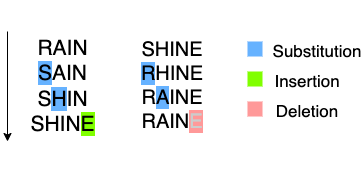
\includegraphics[width=8cm,height=3.5cm]{chapters/figures/Leven.png}
    \caption{Example showing Levenshtein distance calculation}
    \label{fig:Levenshtein}
\end{figure}

We use the Python Fuzzy-Wuzzy\footnote{https://pypi.org/project/fuzzywuzzy/} library which uses Levenshtein distance to calculate the similarity between two strings. 

We calculate the Levenshtein distance between the tokenized keywords $KW_{Q}$ in the question and the list of relations $\mathcal{R}_{DB}$ obtained from Section \ref{sec:relationsfromdbpedia}. 
The top-k candidate relations are retrieved using the following method: 
\begin{enumerate}
    \item We split the relations in $\mathcal{R}_{DB}$ into tokens as some relations in DBpedia are a sequence of concatenated tokens, as shown in Table \ref{tab:relations}.
    \item We extract the keywords in the question $KW_{Q}$ using the techniques in Section \ref{sec:preprocessnlq}. Finally, the Levenshtein distance between each keyword and the tokens in the KG relations are calculated.
    \item We retrieve the top-k relations based on the minimum distance calculated.
\end{enumerate}

\begin{table}[H]
    \centering
    \begin{tabular}{|c|c|}
     \hline
     \textbf{Relations from DBpedia} & \textbf{Split Relations} \\
    \hline
     foundedBy & founded By \\
    \hline
    associatedMusicalArtist & associated Musical Artist \\
    \hline
    foundingYear & founding Year \\
    \hline
    \end{tabular}
    \caption{Relations in DBpedia}
    \label{tab:relations}
\end{table}

\textbf{Jaro Similarity}. The Jaro distance is a measure of edit distance between two strings. Jaro Similarity is the inverse of the Jaro distance. Jaro Similarity compares two strings and gives a score representing how similar they are. It counts the characters that match between the two strings irrespective of the location, provided they are close to each other.

The Jaro similarity sim\_{j(a,b)} of two given strings a and b is give by

\begin{singlespace}
\begin{equation}
   sim_{j(a,b)} = \left\{ \begin{array}{cl}
0 & \ if \ m = 0 \\
\frac{1}{3} \left(  \frac{m}{|a|}+\frac{m}{|b|}+\frac{m-t}{m}\right)& otherwise
\end{array} \right. 
\end{equation}
\end{singlespace}

\begin{quote}
Where, \\
$|a|$ is the length of string a, \\
$|b|$ is the length of string b, \\
m is the number of similar characters, \\
t is the half the number of transpositions.
\end{quote}
Transpositions is defined as the number of matching characters
that are in a different order, divided by 2, provided they are not $\left\lfloor \frac{max(|a|,|b|)}{2} \right\rfloor - 1$ positions apart.

If two strings have completely different characters, then \textit{m = 0} and \textit{$sim_{j(a,b)} = 0$}.
If two strings are exactly the same, then 
\textit{m = $|a|$ = $|b|$} and \textit{t = 0}, hence, \textit{$sim_{j(a,b)} = 1$}.

The Jaro distance is given by,
\begin{equation}
    dist_{j}=1-sim_{j}
\end{equation}

Let us consider the strings, a=RAIN (length=4) and b=SHINE (length=5), "I" and "N" appear in both strings and in the same order, thus, no transpositions are needed. Therefore, m=2 and t=0. 
The calculation of Jaro similarity of strings a and b is shown below 
% \begin{figure}
%     \centering
%   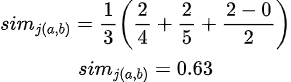
\includegraphics[width=4cm,height=1.5cm]{chapters/figures/jaro.png}
%     \caption{Example showing Jaro similarity calculation}
%     \label{fig:Levenshtein}
% \end{figure}
\begin{quote}
\centering
$sim_{j(a,b)}=\frac{1}{3} \left(  \frac{2}{4}+\frac{2}{5}+\frac{2-0}{2}\right)$ \\
$sim_{j(a,b)}=0.63$
\end{quote}

\textit{Jaro-Winkler similarity} is a modified form of Jaro similarity that increases the score by a constant if the first characters of both strings are the same. 

\begin{singlespace}
\begin{equation}
   sim_{jw(a,b)} = sim_{jw(a,b)} + lp(1-sim_{j(a,b)})
\end{equation}
\end{singlespace}

\begin{quote}
Where, \\
$sim_{j(a,b)}$ is the Jaro similarity of strings a and b, \\
$l$  is the length of common prefix at the start of the string up to a maximum of 4 characters, \\
$p$ is a constant scaling factor for how much the score is adjusted upwards for having common prefixes. The standard value for this constant is 0.1
\end{quote}

The Jaro-Winkler distance is given by,
\begin{equation}
    dist_{jw}=1-sim_{jw}
\end{equation}

If there are no common prefixes the Jaro similarity and the Jaro-Winkler similarity return the same similarity score.

We use the Python Jaro-Winkler\footnote{https://pypi.org/project/jaro-winkler/} library to calculate the Jaro similarity and the Jaro-Winkler similarity  between two strings. 

We calculate the Jaro similarity between the tokenized keywords $KW_{Q}$ in the question and the list of relations $\mathcal{R}_{DB}$ obtained from Section \ref{sec:relationsfromdbpedia}. 
The top-k candidate relations are retrieved using the following method: 
\begin{enumerate}
    \item We split the relations in $\mathcal{R}_{DB}$ into tokens as some relations in DBpedia are a sequence of concatenated tokens, as shown in Table \ref{tab:relations}.
    \item We extract the keywords in the question $KW_{Q}$ using the techniques in Section \ref{sec:preprocessnlq}. Finally, the Jaro similarity and the Jaro-Winkler similarity between each keyword and the tokens in the KG relations are calculated.
    \item We retrieve the top-k relations based on the similarity score.
\end{enumerate}

The similarity score is between \textbf{0} and \textbf{1}, where 0 means the strings are entirely different and
1 means they match exactly.

\subsection{Word Embeddings}
\label{sec:wordembeddings}
Word embedding techniques such as Word2vec\cite{word2vec}, FastText\cite{fasttext} and Glove\cite{glove} learn a numerical representation for words such that words that have the same meaning have a similar representation. Embeddings are dense vectors of floating point values which are trainable parameters. The weights are learnt by the model during training. Word embeddings are created by training a collection of fixed-length, dense and continuous-valued vectors on a huge corpus of text. A higher dimensional embedding can capture fine-grained relationships between words, but takes more data to learn. Each word in a word-embedding is represented by a point in the embedding space, which is learnt and moved based on the surrounding words. Word vectors are constructed based on the distance between each vector in the vector space. 

Contextual representations of language are functions that leverage the idea that the meaning of a particular word in a particular text depends not only on the identity of a word, but also on the words that surround it at that moment. The most popular Contextualized (Dynamic) Word Embedding techniques are BERT\cite{bert}, ElMo\cite{elmo} etc.

We analyzed two word-embedding techniques on the relations obtained from DBpedia: Word2vec and BERT.

\textbf{Word2vec.} Word2vec is one of the most popular word embedding techniques used in natural language processing. It is a feed-forward neural network with just one hidden layer. Hence, it is referred to as a Shallow Neural Network architecture. Pre-trained Word Embeddings capture the semantic and syntactic meaning of a word as they are trained on large datasets. The pre-trained Google Word2vec\footnote{https://code.google.com/archive/p/Word2vec/} model is trained on Google news data (about 100 billion words), it contains 3 million words and phrases and is fit using 300-dimensional word vectors. We use the pre-trained Word2vec model for our evaluation.

Word2vec model computes the word vector for a single token. When a token is converted to its vector representation in Word2vec, we check if that token is present in the Word2vec vocabulary. Tokens that are not present in the vocabulary (out-of-vocabulary words) are \textbf{not considered}. As some relations in DBpedia are a sequence of concatenated tokens, as shown in Table \ref{tab:relations}, we calculate the mean value of the vectors of the tokens to represent the relation as a single vector.

Consider an example relation, \textbf{associatedMusicalArtist}. The relation is an out-of-vocabulary word in the Word2vec model. We first spilt the relation into the following tokens, \textbf{associated}, \textbf{musical}, \textbf{artist}. We then convert the tokens to their corresponding vectors v1, v2 and v3 respectively and calculate the mean of the vectors. The mean of the vectors is given by
\begin{equation}
    m(n) = \frac{ v(1) + v(2) + ... + v(n)}{n}
\end{equation}
where, n is the number of tokens.

To find the similarity between the strings, we compute the cosine similarity, which is given by the dot product of the  vectors of the strings $\mathcal{A}$ and $\mathcal{B}$. The cosine similarity is given as follows,
\begin{equation}
    cosine_{sim}(\mathcal{A},\mathcal{B}) = \frac{\mathcal{A} \cdot \mathcal{B}}{||\mathcal{A}||\ ||\mathcal{B}||}
\end{equation}
where, $\mathcal{A}$ and $\mathcal{B}$ are the vectors of the strings, and $||\mathcal{A}||$ and $||\mathcal{B}||$ are the length of the two vectors $\mathcal{A}$ and $\mathcal{B}$

The top-k candidate relations are retrieved using the following method: 
\begin{enumerate}
    \item We split the relations in $\mathcal{R}_{DB}$ into tokens. Each of these tokens are converted into their corresponding vector representation and the mean of these vectors is calculated.
    \item  We extract the keywords in the question $KW_{Q}$ using the techniques in Section \ref{sec:preprocessnlq}. Each of these keywords are converted into their corresponding vector representation.
    \item Finally, the cosine similarity between each keyword and the mean vector that represents each relation in the KG relations $\mathcal{R}_{DB}$ are calculated. 
    \item We retrieve the top-k relations based on the cosine similarity score calculated.
\end{enumerate}

\textbf{BERT Embeddings.} BERT or Bidirectional Encoder Representation from Transformers, is a natural language processing pre-training developed by Google. BERT uses transformer architecture to learn embeddings for words. It is designed to pre-train deep bidirectional representations from unlabeled text including Wikipedia and Book corpus by jointly conditioning on both left and right context in all layers. BERT offers an advantage over models like Word2Vec as BERT produces word representations that are dynamically informed by the words around them while in Word2Vec each word has a fixed representation of the context within which the word appears.

We implement the BERT embedding technique using the sentence-transformers library from Python which uses HuggingFace\footnote{https://huggingface.co/sentence-transformers/bert-base-nli-mean-tokens} transformers. We use the pre-trained \textit{bert-base-nli-mean-tokens} model has 12 layers (transformer blocks), 12 attention heads, 110 million parameters and a hidden size of 768. We have approximately 54,000 relations from DBpedia. We get 54,000 embeddings each containing 768 values.

The top-k candidate relations are retrieved using the following method: 
\begin{enumerate}
    \item We split the relations in $\mathcal{R}_{DB}$ into tokens. The split tokens are encoded to get their corresponding embeddings.
    \item  We extract the keywords in the question $KW_{Q}$ using the techniques in Section \ref{sec:preprocessnlq}. Each of these keywords are encoded to obtain their corresponding embeddings.
    \item Finally, the cosine similarity between each encoded keyword and encoded tokens that represents each relation in the KG relations $\mathcal{R}_{DB}$ are calculated. 
    \item We retrieve the top-k relations based on the cosine similarity score calculated.
\end{enumerate}

The resulting similarity ranges from $-1$ to 1, where 1 means exactly the same, 0 means less similar and in-between values indicate intermediate similarity or dissimilarity.

\subsection{Term Frequency-Inverse Document Frequency}
\label{sec:tfidf}
Term Frequency - Inverse Document Frequency (TF-IDF) has the underlying concept that if a term (keyword) occurs more than once in a document, then that word is significant for that document. Also, if a term (keyword) occurs a number of times in many documents, then that term (keyword) is insignificant. The score produced by TF-IDF is based on considering the above two ideas of the frequency of occurrence of a term (keyword). 

\textbf{Term Frequency.} Term Frequency of a keyword in a document is the raw count of the keywords that appear in a document. We calculate the term frequency of a keyword using the $List_{r}$ (document) obtained in Section \ref{sec:TextCleaningPipeline}, Algorithm \ref{alg:dictcreation} (line 7).
\begin{equation}
Term \ Frequency, \ TF_{r} = \frac{count \ of \ keyword \ in \ List_{r}}{number \ of \ keywords \ in \ List_{r}}
\end{equation}
\textbf{Inverse Document Frequency.}
Inverse document frequency is used to find how common a keyword is amongst all the documents. To calculate the Document Frequency (DF) for all the keywords present in the $List_{r}$ (document) for each relation, we create a hashmap, whose key is the keyword present across all the $List_{r}$ (documents) and the value is the count of $List_{r}$ (documents) where the keyword occurs.

The Document Frequency, $DF_{keyword}$ and Inverse-Document Frequency, $IDF_{keyword}$ is given as follows
\begin{equation}
   DF_{keyword} = occurrences \ of \ keyword \ in \ N \ keyword\_List_{r}
\end{equation}
\begin{equation}
      IDF_{keyword} = log\left( \frac{N}{(DF+1)} \right)
\end{equation}
where, r is a relation in $\mathcal{R}_{DB}$ and  N is the total number of relations present in $\mathcal{R}_{DB}$. We use the logarathmic inverse while calculating IDF as the N value is large such that it dampens the importance of term that has a high frequency. 

The TF-IDF for a relation r and a keyword is a hashmap, whose key is relation-keyword pair and the value is the TF-IDF score, which is given by
\begin{equation}
      TF-IDF \ [r,keyword] = TF_{r}*IDF_{keyword}
\end{equation}

The top-k candidate relations are retrieved using the following method: 
\begin{enumerate}
    \item  We extract the keywords in the question $KW_{Q}$ using the techniques in Section \ref{sec:preprocessnlq}. Each of these keywords are searched in the key of the TF-IDF hashmap.
    \item We retrieve the top-k relations based on TF-IDF scores returned for each keyword.
    % \item Finally, the cosine similarity between each keyword and the mean vector that represent each relation in the KG relations $\mathcal{R}_{DB}$ are calculated. 
    % \item We retrieve the top-k relations based on the cosine similarity score calculated.
\end{enumerate}
Let us consider an example keyword "bear" (lemmatized form of born), we check in every document if this keyword exists and if the keyword exists, then the TF-IDF value is returned for that particular relation (the document where it occurs). We sort the TF-IDF scores and display the top k relations. The top-5 relations returned for the keyword "bear" are \textit{cityOfBirth, nationality(ethnicOrigin), yearOfBirth, countryOfBirth} and \textit{originally}.

\section{Results}
In this section, we discuss the results from the experiments over our datasets and baselines.

We first evaluate the Hits@k (k=5, 10, 15) results of ReMLOFT and the other baselines. We compare the performance of our system with 5 other techniques, Levenshtein distance, Jaro similarity, Jaro-Winkler similarity, Word2vec, BERT and TF-IDF. Figure \ref{fig:top5hits} shows the Hits@5, Figure \ref{fig:top10hits} shows the Hits@10 and Figure \ref{fig:top15hits} shows the Hits@15 for the QALD datasets across all the baselines. We notice that the Hits@k increases significantly when k is increased across all the datasets. 
As the complexity of the question increases, the number of expected relations to build a SPARQL query increases. 
Increase in k in ReMLOFT yeilds better results due to the noisy nature of the information-dense free-text knowledge graph.


\begin{figure}[p]
    \centering
    \begin{minipage}{0.7\textwidth}
   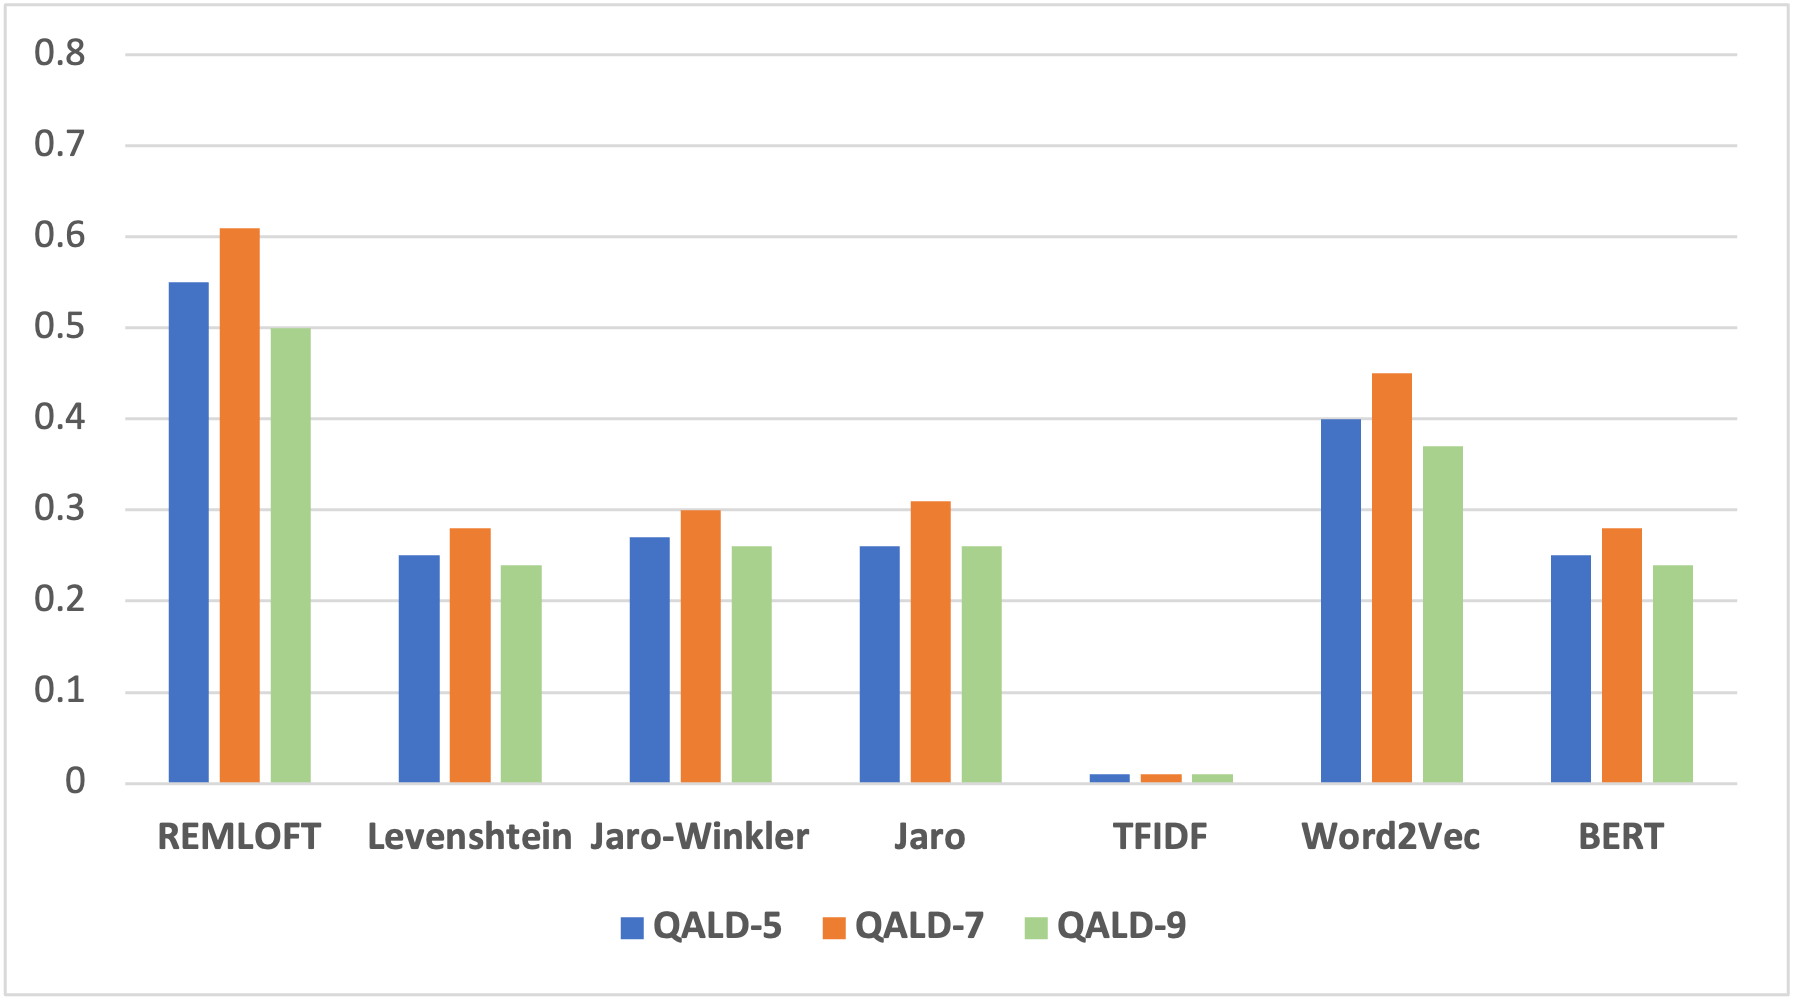
\includegraphics[width=\textwidth]{chapters/figures/top5bert.png}
    \caption{Hits@5 ReMLOFT vs other baselines}
    \label{fig:top5hits}
     \end{minipage}
         \begin{minipage}{0.7\textwidth}
   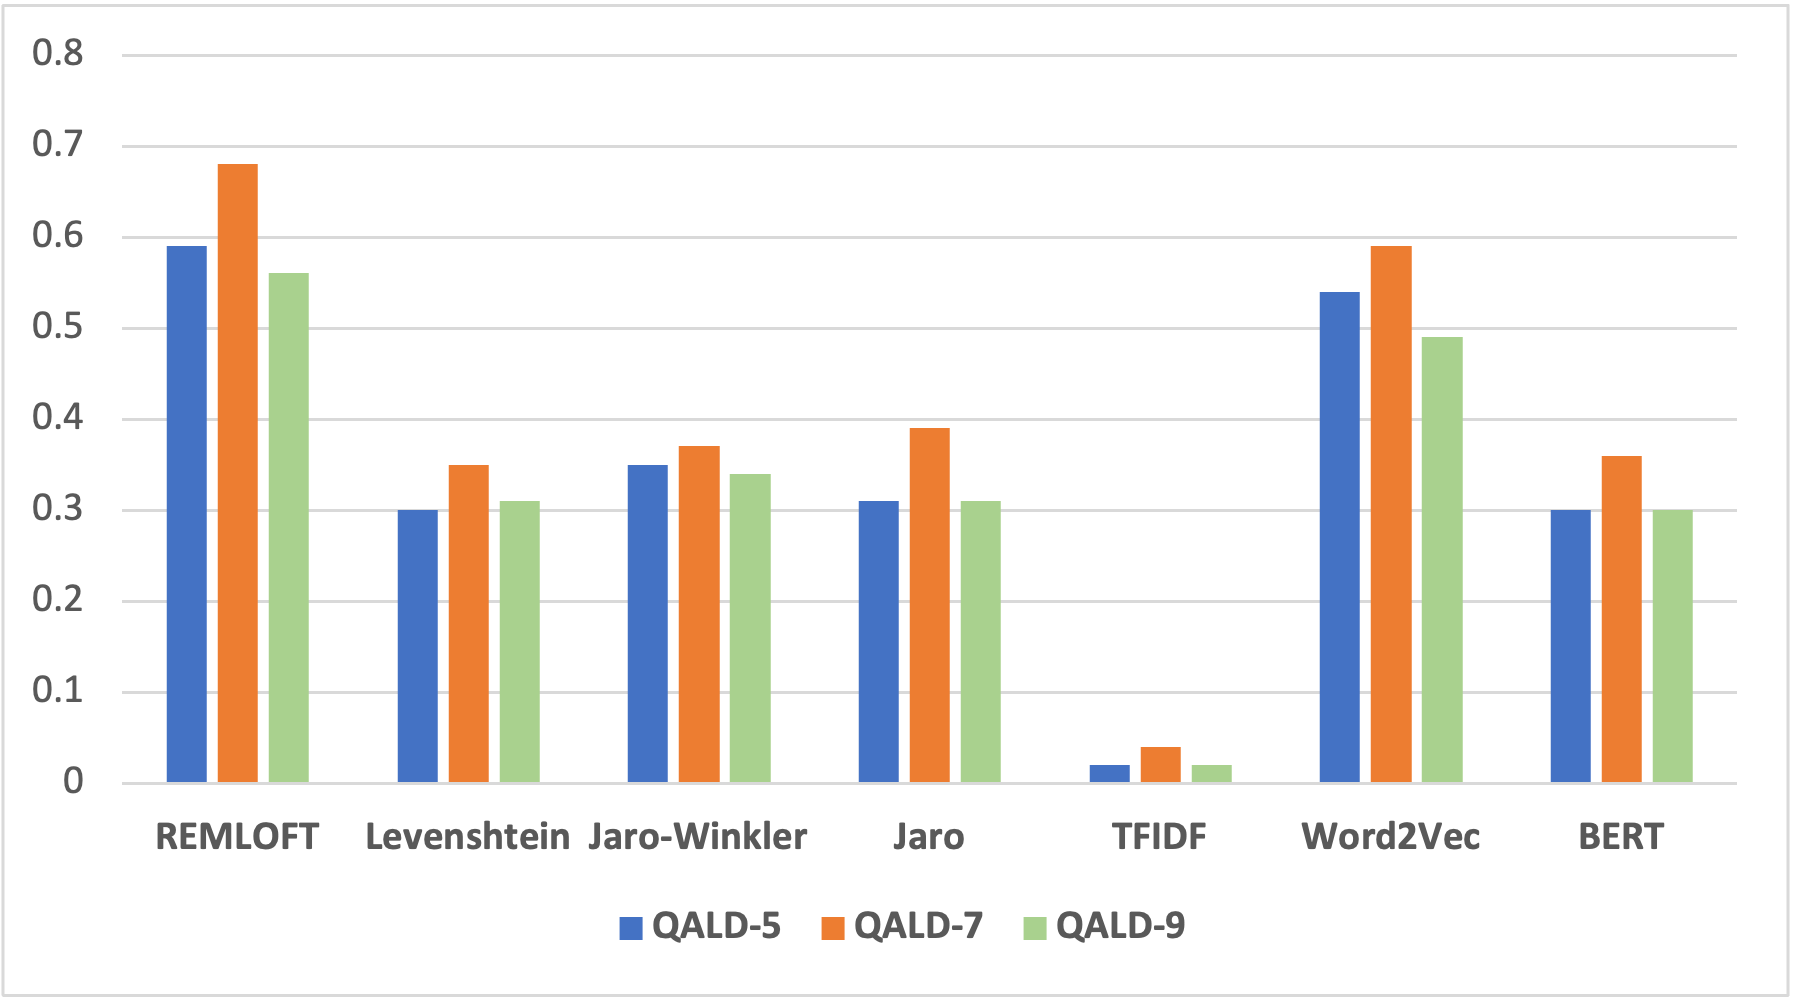
\includegraphics[width=\textwidth]{chapters/figures/top10bert.png}
    \caption{Hits@10 ReMLOFT vs other baselines}
    \label{fig:top10hits}
     \end{minipage}
         \begin{minipage}{0.7\textwidth}
    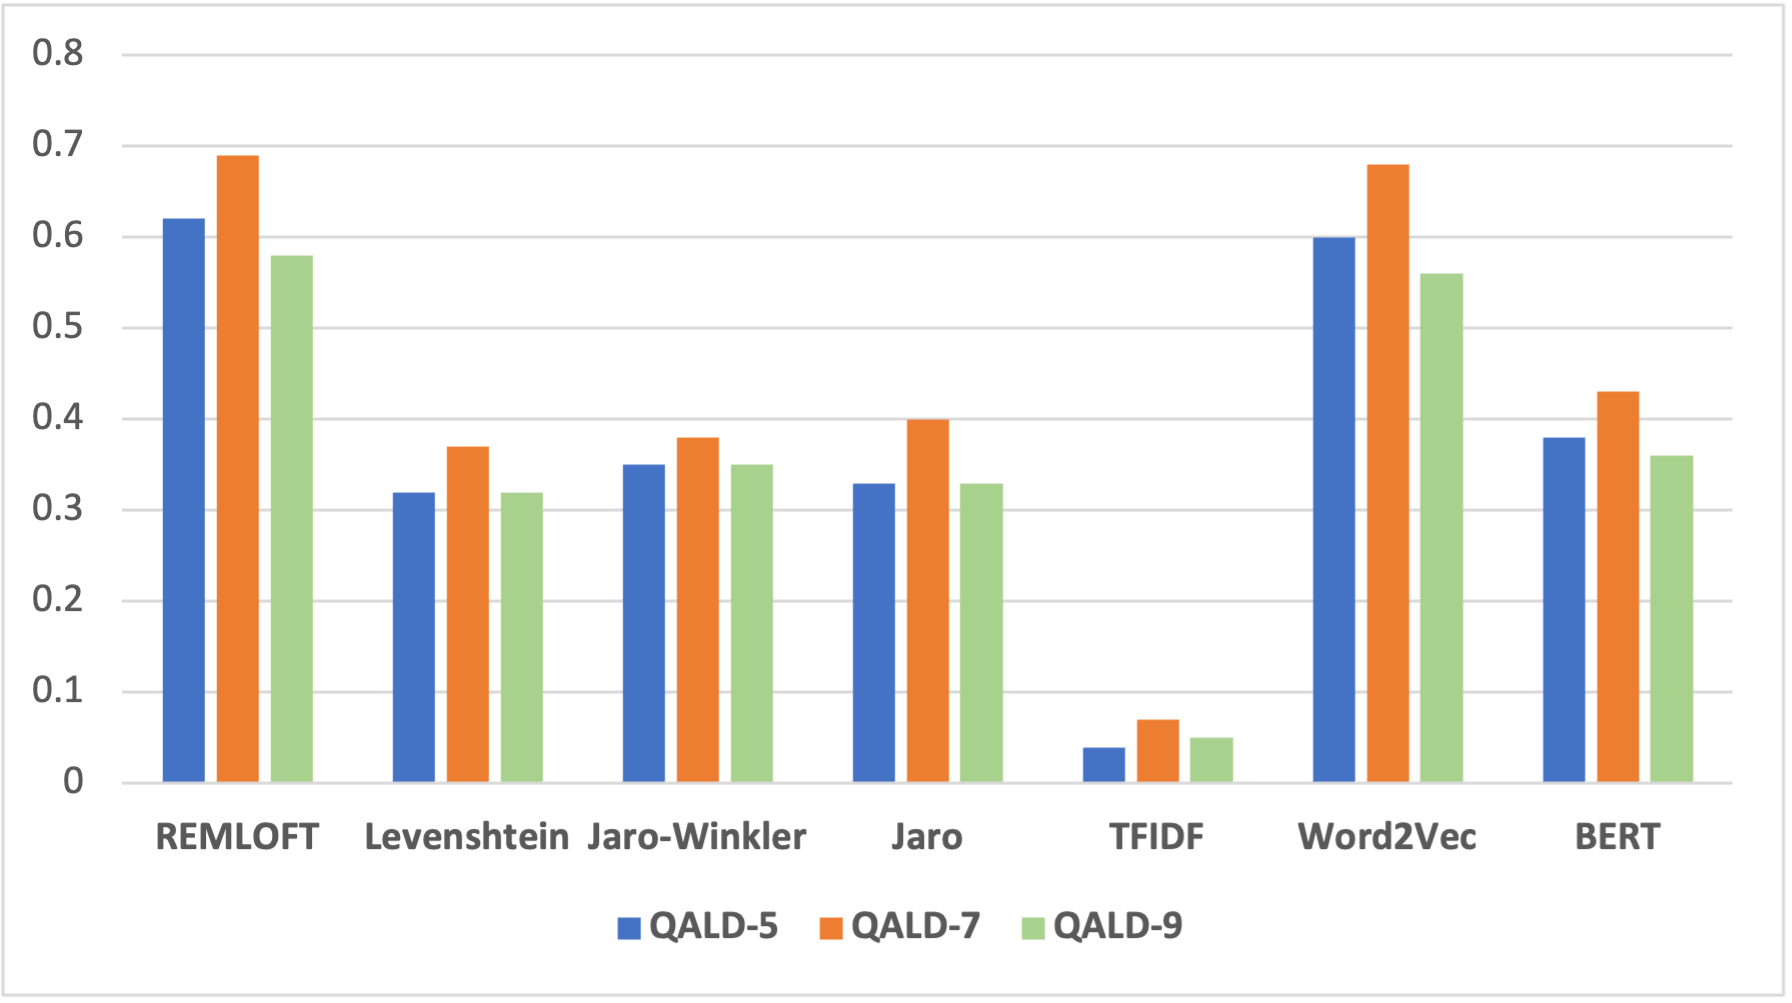
\includegraphics[width=\textwidth]{chapters/figures/Top15Bert.png}
        \caption{Hits@15 ReMLOFT vs other baselines}
        \label{fig:top15hits}
    \end{minipage}
\end{figure}


Both string similarity and word embedding methods are used on the list of relations $\mathcal{R}_{DB}$. Though string similarity is practical for words with spelling errors or plural forms of words, they do not capture the semantics of the keyword. String similarity techniques are successful for questions such as \textit{Who developed Slack?}, expected relation: \textit{developer}, where the keyword \textit{develop} is used for the search,
but \textbf{fail} to answer questions like \textit{Who is the host of the BBC Wildlife Specials?} where the expected relation: \textit{presenter} cannot be matched with the keyword \textit{host}. 

To overcome the limitation of the string similarity techniques used, we use the pre-trained word embeddings from Word2vec. We observe a significant increase in the Hits@k value. This is because word embeddings capture the semantics of the relations, thereby returning semantically similar relations. Word2vec represents every word as an independent vector and thus we compute the mean of the word vectors to receive a single vector. Averaging of vector representations using pre-trained word embeddings results in the loss of information. The pre-trained word embedding approach has the constraint of out-of-vocabulary words. Some of the tokens mentioned in the relations are not found in the Word2Vec vocabulary. When the model encounters a new word, it skips the word, thereby making it less ideal to capture the similarity of the keyword. Though word-embeddings give satisfactory results, they cannot be extended to other domains unless the word embedding is trained using specific domain vocabulary.

Word-level similarity comparisons are not appropriate with BERT embeddings because these embeddings are contextually dependent, meaning that the word vector changes depending on the sentence it appears in. Contextually dependent vectors can be obtained only in the sentence-level and not in the word-level similarity. Since we compare each keyword in the question with the relations from DBpedia, BERT doesn't give exceptional results. 

We also evaluate the TF-IDF on the free-text KG. We observe that the TF-IDF method performs unsatisfactorily as compared to the other methods used. This is due to the large frequency of certain words in the relation documents. For a given keyword k, if we consider there are 10,000 documents that contain the keyword and 1000 documents that do not contain the keyword, the inverse document frequency of k is very low (because it is found in almost all documents), and k gets a very small TF-IDF score. The same argument applies for TF, given 2 documents - one consisting of 100 unique words, and the other of 1000 unique words, each word in the first document will have a TF of 0.01 while in document 2 each word will have a TF of 0.001 which casues the TF for each document to have a large bias.

\begin{table}[H]
    \centering
    \begin{tabular}{|c|c|c|c|c|}
     \hline
     \textbf{No of Relations} & \textbf{QALD-5} & \textbf{QALD-7} & \textbf{QALD-9}  \\
    \hline
     1 Relation & 0.65 & 0.71	& 0.61 \\
    \hline
    2 Relations & 0.83 & 0.83 & 0.80 \\
    \hline
    3 Relations & 0.63 & 1	& 0.83 \\
    \hline
    4 Relations & 1 & - & 0 \\
    \hline
        Total Coverage & 0.69 & 0.74 & 0.65 \\
            \hline
    \end{tabular}
    \caption{ReMLOFT Coverage for Questions based on the number of relations}
    \label{tab:relationcoverage}
\end{table}

We then evaluate the Coverage of ReMLOFT for the QALD datasets as shown in Table \ref{tab:relationcoverage}. ReMLOFT performs exceptionally for complex questions with more than one relation and has adequate coverage for simple questions. We see that ReMLOFT performs well for questions with two relations across all the datasets with nearly \textbf{80\%} coverage. 
\begin{figure}[h]
    \centering
   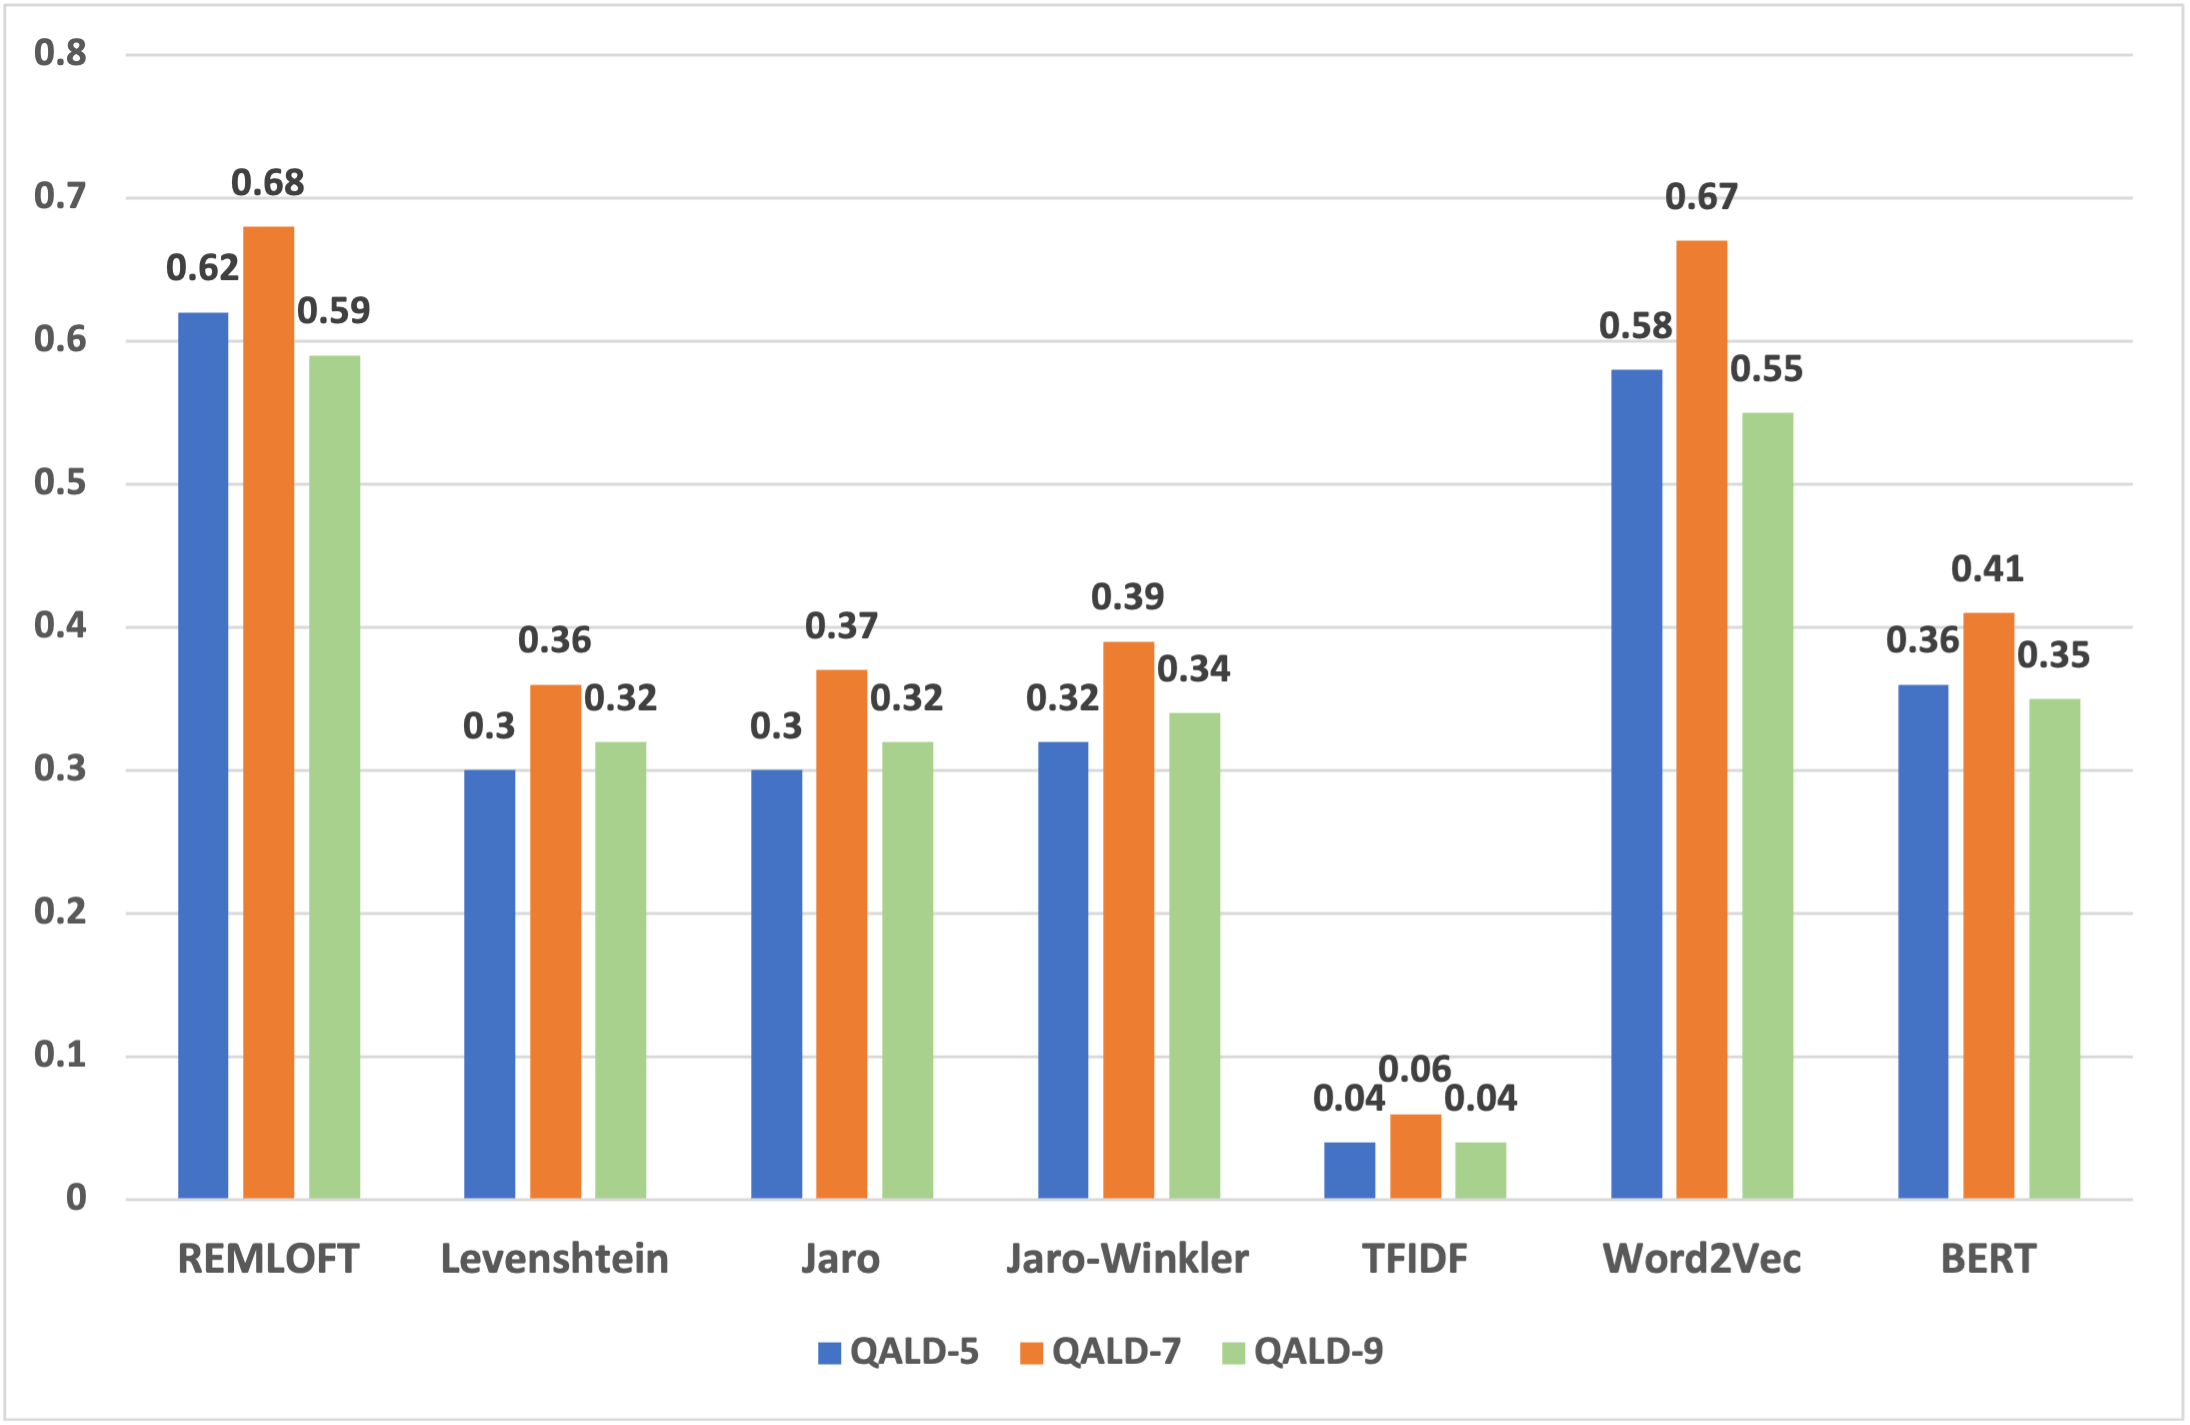
\includegraphics[width=10cm, height=6cm]{chapters/figures/accuracyBert.png}
    \caption{Accuracy of ReMLOFT vs other baselines}
    \label{fig:graphacc}
\end{figure}

We evaluate the accuracy of ReMLOFT in comparison with the other baselines. We observe that the accuracy of ReMLOFT varies based on the number of questions in the dataset. ReMLOFT returns 163 relations from a total of 262 relations for QALD-5, 142 relations from a total of 209 relations for QALD-7 and 259 relations from a total of 441 relations for QALD-9. Figure \ref{fig:graphacc} shows that ReMLOFT represents a vast improvement in accuracy when compared to the baselines.

In conclusion, ReMLOFT performs better than the baseline techniques to map relations, especially for questions with multiple expected relations. 

\section{Limitations}
In this section, we investigate the shortcomings of our approach.

\textbf{Missing Entity.} Some questions found in the QALD dataset do not have an entity. For example, {\fontfamily{pcr}\selectfont Which countries have more than two official languages?}, has no given entity. Our approach relies on the relations returned by DBpedia entities to reduce the the number of candidate relations. Therefore, questions without an entity don't return a result even though the keywords from the question return valid relations from the Free-text KG. The candidate relations from the Free-text KG is a large search space. Hence, pruning the necessary candidate relations would require extensive filtering. 

\textbf{Insufficient Keywords.} ReMLOFT does not work effectively if there are not enough keywords in the question that describes the context of the question. 
Consider the following example questions below,
\begin{enumerate}
    \item \textbf{Where in France is sparkling wine produced?}, has two gold standard entities, \textit{"sparkling wine"} and \textit{"France"}. However, the keyword \textbf{produce}, is not sufficient to return the expected relations \textit{wineProduced} and \textit{location}. 
    \item \textbf{Was Margaret Thatcher a chemist?}, with the gold standard entities \textit{"Margaret Thatcher"} and \textit{"chemist"}. We are left with \textit{no keywords} to evaluate the question.
\end{enumerate}

Including the entities as keywords for mapping relations from the free-text KG could overcome this problem, but this would introduce a lot of noise and increase the number of candidate relations to filter from.

\textbf{Semantic Significance.} Though our approach captures the semantics of a specific word using the knowledge from the Free-text KG. It does not always imply the top ranking of the correct relations for certain keywords. A keyword could be closely related to another relation than the expected gold standard relations.
Consider the question, \textbf{How much did Pulp Fiction cost?}, where the expected gold standard relation is \textit{budget}. The keyword \textbf{cost} maps to the relations \textbf{cost} and \textbf{netIncome} as the top two relations from the free-text KG.

\textbf{Effect of n-grams.} Since our approach uses unigrams, keywords that are n-grams do not work effectively. A keyword \textbf{timezone} returns less significant relations as compared to \textbf{time zone} which returns the expected gold standard relation.

